\documentclass[a4paper]{article}
\usepackage{amsfonts}
\usepackage{amsmath}
\usepackage{amsthm}
\usepackage[utf8]{inputenc}
\PassOptionsToPackage{hyphens}{url}\usepackage{hyperref}
\usepackage{booktabs}
\usepackage{graphicx}
\usepackage{listings}
\usepackage{float}
\usepackage{siunitx}
%\usepackage{subcaption}

\graphicspath{ {fig/} }

\title{Lab 4: Support Vector Machines}
\author{Santiago Bernal \\ Rodrigo Arias}

\begin{document}
\maketitle

\section{Exercise 1}
%
% 1. Download from racó a python file named `exercise1_svm.py` in which you have
% to analyze three simple data sets.
%
In the file \texttt{ex1.py} three generators are used to provide 3 different 
random datasets.
%
% 2. For each data set you have a corresponding python function. In this
% function, you will call a SVM algorithm with three kernel functions. You will
% plot the hyperplane that separate the data set and its support vectors.
%
The SVM algorithm is applied to the train set of each dataset, and is plotted in 
the figures~\ref{fig:ex1gen1}, \ref{fig:ex1gen2} and~\ref{fig:ex1gen3}.
%
% 3. Make a prediction for the test data set with the SVM classifier and, in the
% console, write the number of instances correctly predicted and the total number
% of instances to predict. You can use sklearn library and the SVM algorithm
% included on it inside your python function.
%
The train data is shown with circle markers, while the test data uses crosses.  
The SVM decision regions are also filled with color, in order to visually see 
the behavior of the classifier.
%
% 4. In the report, for each one of the data sets, plot the different kernel
% functions analyzed and justify which is the best option for each one of them,
% taking into account that each data set has a different linear distribution.
%

We see that the datasets 1 and 3 are linearly separable, so a linear function 
should be used. The Gaussian kernel is used in the latter, but is behaving 
similarly to a linear kernel, so the classification is correct. The dataset 2, 
in contrast, is clearly not linearly separable, so a linear function should not 
be used. In the figure~\ref{fig:ex1gen2a} a Gaussian kernel was used, to see the 
difference. We see a better classification as expected.

The figure~\ref{fig:ex1gen2} shows a correct classification of 100\%, even if 
the classifier is not accurate. That can be explained because the test set 
provided with the generator, is only choosing elements that are placed in the 
outermost groups.
%
\begin{figure}[H]
	\centering
	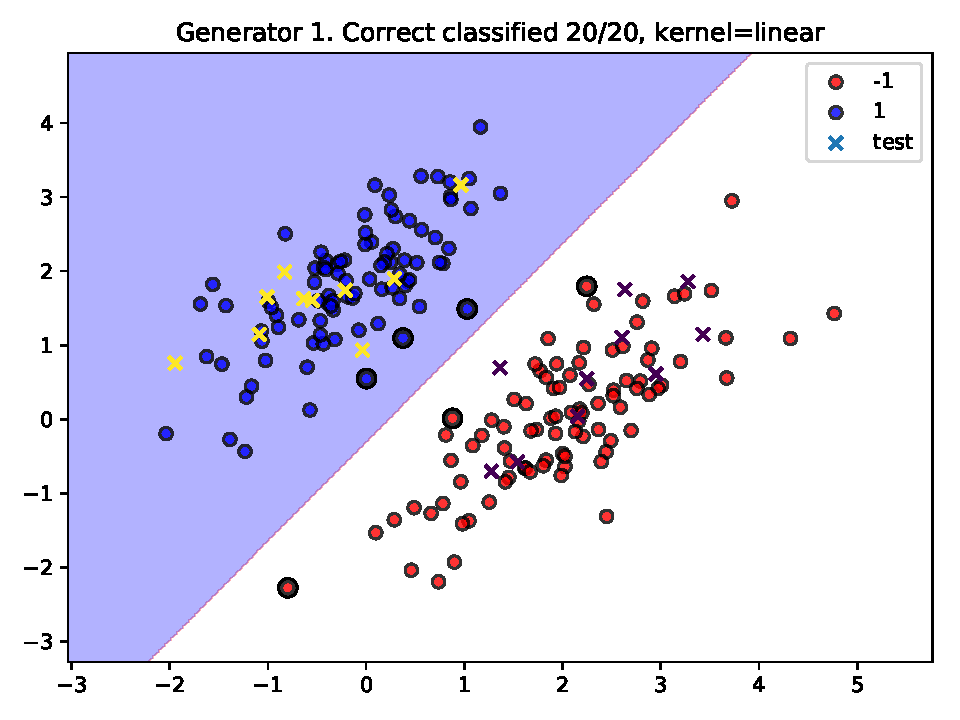
\includegraphics[width=0.7\textwidth]{ex1/1.pdf}
	\caption{Dataset of the generator 1}
	\label{fig:ex1gen1}
\end{figure}
\begin{figure}[H]
	\centering
	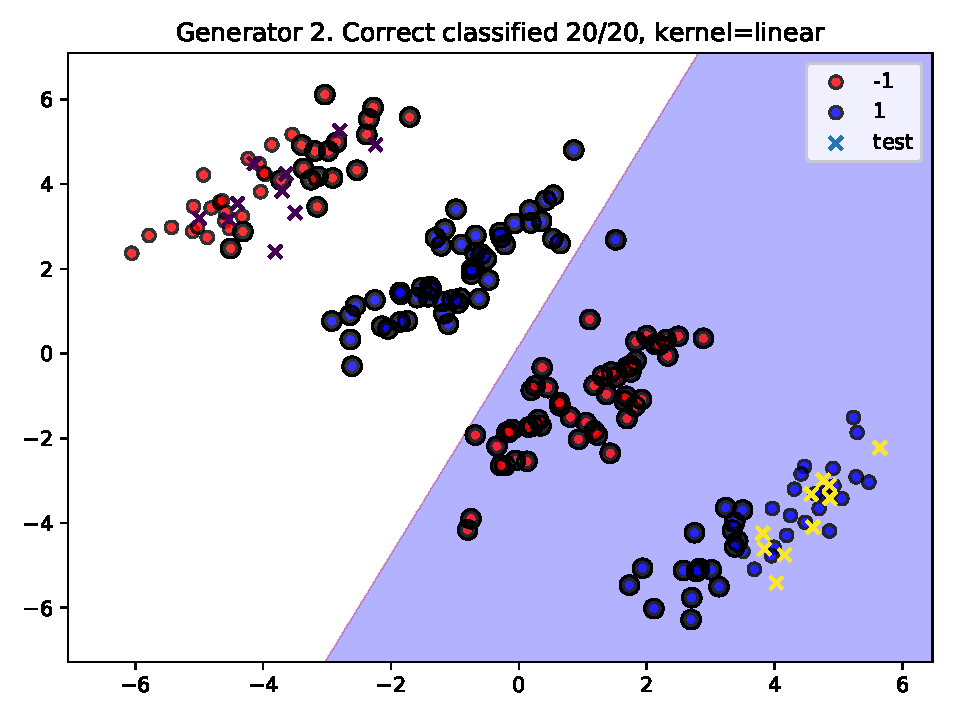
\includegraphics[width=0.7\textwidth]{ex1/2.pdf}
	\caption{Dataset of the generator 2}
	\label{fig:ex1gen2}
\end{figure}
\begin{figure}[H]
	\centering
	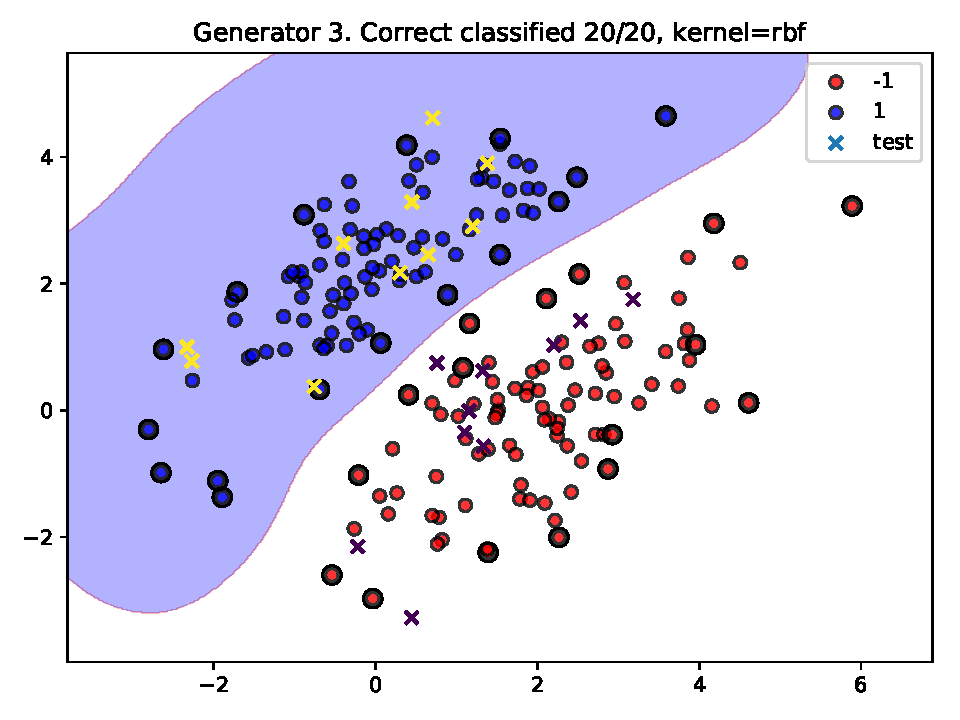
\includegraphics[width=0.7\textwidth]{ex1/3.pdf}
	\caption{Dataset of the generator 3}
	\label{fig:ex1gen3}
\end{figure}
\begin{figure}[H]
	\centering
	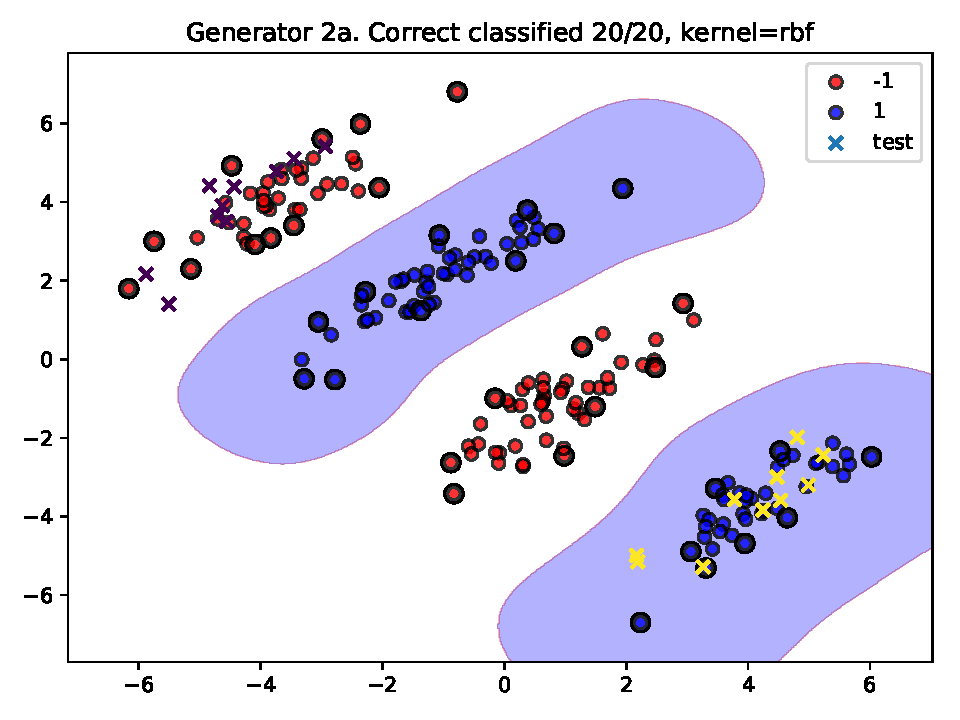
\includegraphics[width=0.7\textwidth]{ex1/2a.pdf}
	\caption{Dataset of the generator 2 using a Gaussian kernel}
	\label{fig:ex1gen2a}
\end{figure}
%

\section{Exercise 2}
%
% 1. Use the parser developed in previous assignment for reading and saving the
% information from a training and their corresponding testing files in arff
% format.
%
In the file \texttt{ex2.py} we adapted the previous parser for ARFF files, to 
read the training and testing datasets.
%
% 2. Use the Python function that automatically repeats the process described in
% previous step for the 10-fold cross-validation files. That is, read
% automatically each training case and run each one of the test cases in the
% selected classifier.
%
% 3. Write a Python function for classifying, using a SVM algorithm, each
% instance from the TestMatrix using the TrainMatrix to a classifier called
% `SVM_Algorithm(...)`.  You decide the parameters for this classifier. You can
% use sklearn library and the SVM algorithm included on it inside your python
% function. Justify your implementation and add all the references you have
% considered for your decisions.
%
The function \texttt{svm\_classify} implements the SVM algorithm, and computes 
the time and score (the accuracy, defined as the number of correct classified 
classes over the total). We only take into account the numeric part of the 
datasets; the nominal features are ignored. Also we scale the data in order to 
facilitate the work to SVM \cite{scikit-tips}.
%
% 4. For the kernel function, you must consider different alternatives (at least
% three, you can use the predefined kernels included in sklearn or implement
% your own as a precomputed kernel in sklearn) and optimize the parameters of
% them to obtain the best results with the SVM algorithm in your data sets. That
% is, each one of the data sets analyzed may have a different set of parameters.
%
For the kernel functions considered we use three of the predefined ones in 
sklearn: \texttt{linear}, \texttt{rbf} (Gaussian), and \texttt{sigmoid}.
%
% a.  For evaluating the performance of the SVM algorithm, we will use the
% percentage of correctly classified instances. This information will be used
% for the evaluation of the algorithm. You can store your results in a memory
% data structure or in a file. Keep in mind that you need to compute the average
% accuracy over the 10-fold cross-validation sets.
%

The result of each configuration for each fold is stored in memory, until all 
results are finally computed. Then we use the mean accuracy of each 
configuration, to reduce the noise. We use the provided folds for the datasets, 
which are divided into 10 groups of folds, so we take the mean of the 10 
results.
%
% At the end, you will have a SVM algorithm with several kernel functions (you
% will choose them) and with different settings in the hyper-parameters of the
% classifier. You should analyze the behavior of these kernel functions and
% parameters in the SVM algorithm and decide which combination results in the
% best SVM algorithm for each data set.
%

First, a quick run with the default values and the different kernel function 
selects the best one. Then each configuration of parameters is build by choosing 
one value for $\texttt{C} \in \{1,4,6,8\}$ and another for $\texttt{cgamma} \in 
\{1,4,5,8\}$. A total of 16 configurations are run for each fold using the best 
kernel as shown in the table~\ref{tab:conf}. The \texttt{gamma} parameter of SVM 
is the division of \texttt{cgamma} by the number of features.
%
\begin{table}[h]
\small
\centering
\begin{tabular}{lcccccccccccccccc}
\toprule
conf. & 1 & 2 & 3 & 4 & 5 & 6 & 7 & 8 & 9 &10 &11 &12 &13 &14 &15 &16 \\
\midrule
\texttt{C} & 1 & 1 & 1 & 1 & 4 & 4 & 4 & 4 & 6 & 6 & 6 & 6 & 8 & 8 & 8 & 8 \\
\texttt{cgamma} & 1 & 4 & 5 & 8 & 1 & 4 & 5 & 8 & 1 & 4 & 5 & 8 & 1 & 4 & 5 & 8 
\\
\bottomrule
\end{tabular}
\caption{The configuration number and the parameters used}
\label{tab:conf}
\end{table}
%
%
% You can compare your results in terms of classification accuracy and
% efficiency.  Extract conclusions by analyzing two data sets (at least one
% should be large).
%

Results are compared in terms of accuracy and efficiency. We selected a small 
dataset \texttt{hepatitis} and a bigger one \texttt{vowel} to perform the 
experiments.


% ### 1.5 Work to deliver
%
% In this work, you will use a SVM algorithm with different kernel functions in
% both exercises to extract conclusions from your analysis. At the end, you will
% find a list of the data sets available for the second exercise.
%
% You will use your code in Python to extract the performance of the different
% combinations Performance will be measured in terms of classification accuracy
% and efficiency. The accuracy measure is the average of correctly classified
% cases. That is the number of correctly classified instances divided by the
% total of instances in the test file. The efficiency is the average
% problem solving time. For the evaluation, in the second exercise, you will use
% a T-Test or another statistical method [1].
%

\subsection{Evaluation}
%
% From the accuracy and efficiency results, you will extract conclusions showing
% graphs of such evaluation and reasoning about the results obtained.
%
% In your analysis, you will include several considerations.
%
% 1. You will analyze the SVM (with different kernel functions). You will
% analyze which is the most suitable combination of the different kernel
% functions analyzed. The one with the highest accuracy. This SVM combination
% will be named as the best SVM.
%
% 2. Once you have decided the best SVM combination. You will analyze it in
% front of using this combination with different hyper-parameters. The idea is
% to improve the SVM algorithm at each one of the algorithms analyzed.
%

In order to compare the accuracy results of each configuration, a statistical 
test can be used to determine if the improvement is significant, or is just 
because of random deviations. A t-test was first considered, but was discarded 
as it would need a pairwise comparison between all pairs of configurations 
\cite{janez}.  An ANOVA test can be used in a group of observations, so it was 
used here.

The null hypothesis is defined as: the mean of all the groups is the same. For 
the first dataset, we obtain a p-value of 1.0, so we cannot reject the 
hypothesis. The box plot in the figure~\ref{fig:box-hepatitis} shows that almost 
all configurations lead to a similar accuracy.

For the dataset vowel, it can be graphically shown in the 
figure~\ref{fig:box-vowel} that some configurations have a very remarkable 
difference. Performing an ANOVA test gives a p-value of \num{5.75E-22} which is 
a very significative. We reject the hypothesis that all the accuracies have the 
same mean.

A more detailed observation can lead to the conclusion that only the 
configurations 1, 5, 9 and 13, the ones with $\texttt{cgamma} = 1$, are 
significatively different from the rest.  If we remove those observations from 
the ANOVA test, we get a new p-value of 0.353.  So we cannot reject that the 
other configurations have the same mean, thus we conclude that there is no 
significant change in the other parameters tested to be produced by a real 
change in accuracy.
%
\begin{figure}[h]
	\centering
	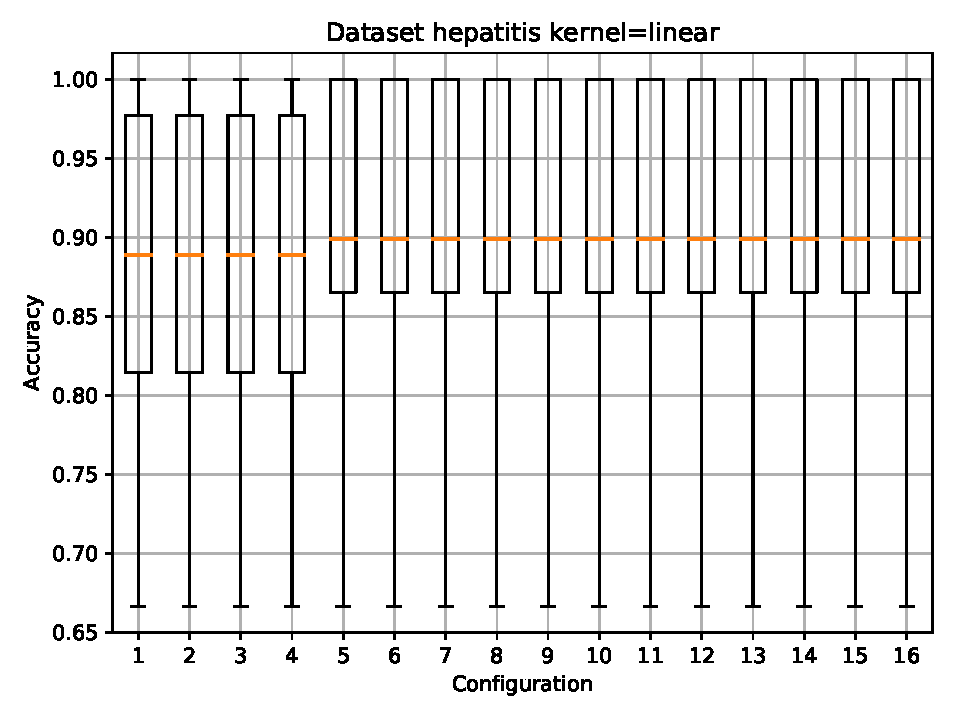
\includegraphics[width=0.49\textwidth]{ex2/hepatitis.pdf}
	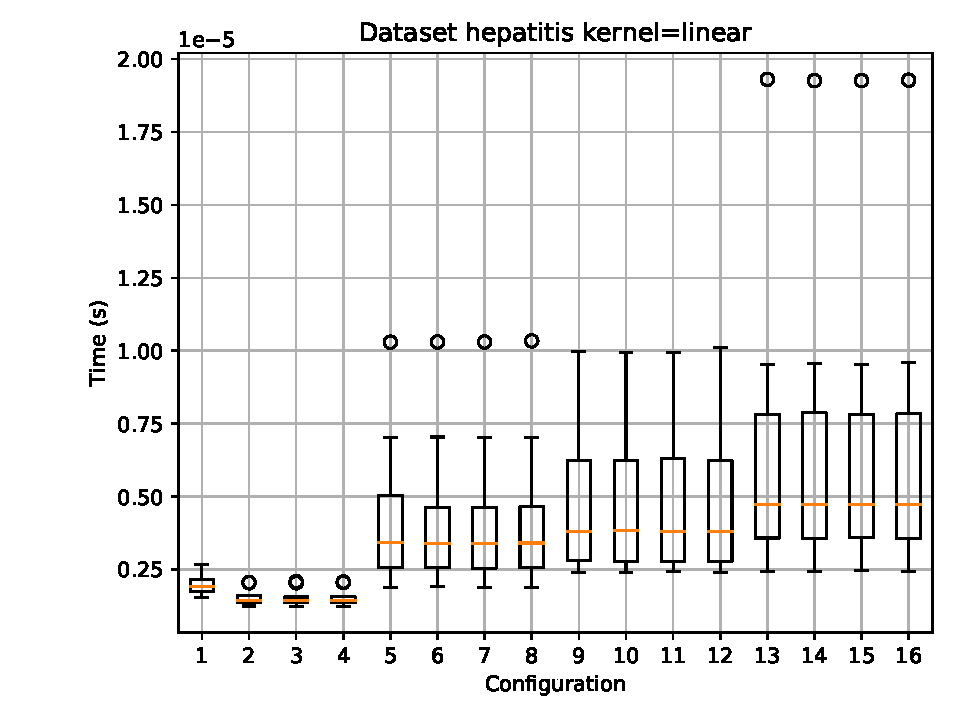
\includegraphics[width=0.49\textwidth]{ex2/hepatitis-time.pdf}
	\caption{Accuracy and time of different configurations for hepatitis}
	\label{fig:box-hepatitis}
\end{figure}
\begin{figure}[h]
	\centering
	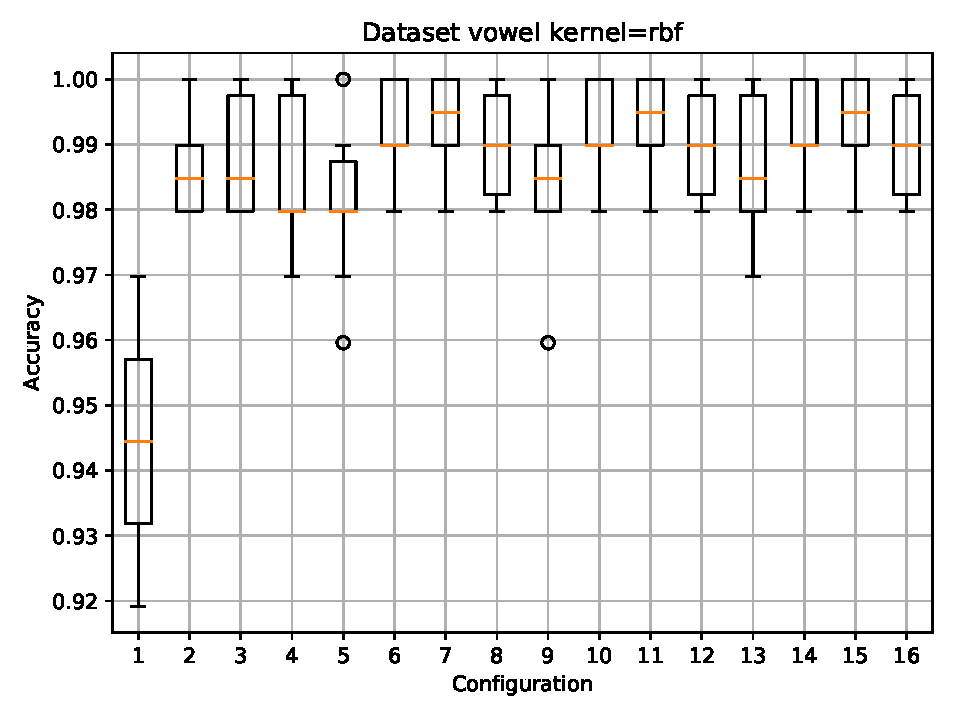
\includegraphics[width=0.49\textwidth]{ex2/vowel.pdf}
	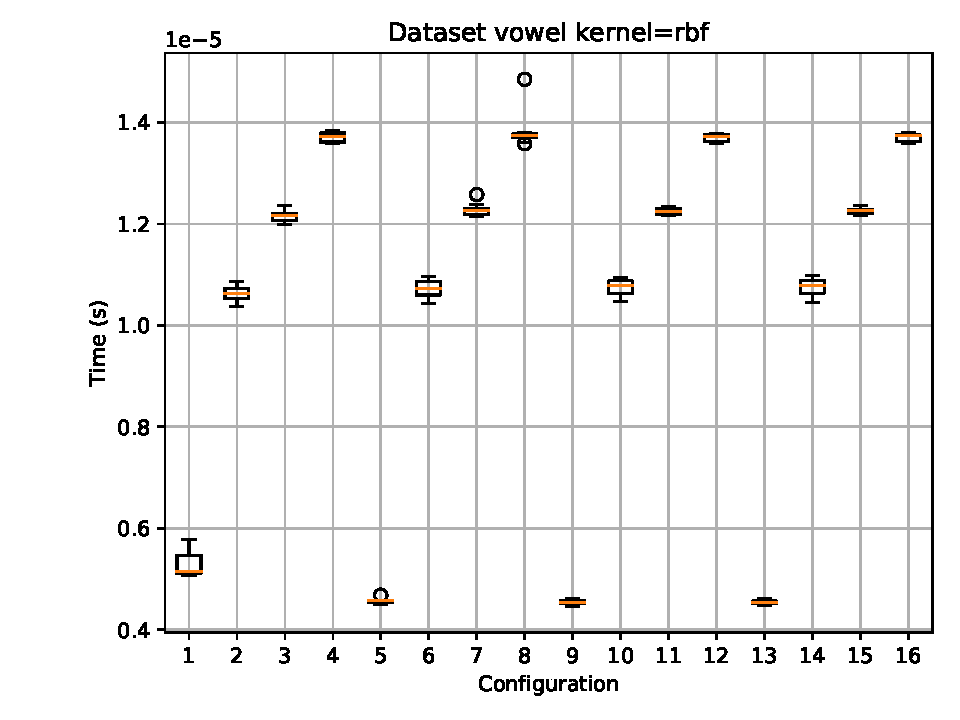
\includegraphics[width=0.49\textwidth]{ex2/vowel-time.pdf}
	\caption{Accuracy and time of different configurations for vowel}
	\label{fig:box-vowel}
\end{figure}

A time analysis reveals that the linear kernel is faster than the Gaussian. The 
time has been scaled by the number of samples and features of each dataset. The 
linear time is around 2 and \SI{5}{\micro\second} while the Gaussian is between 
5 and \SI{14}{\micro\second}

We also observe big fluctuations in time when changing the parameters. The 
linear kernel doesn't take into account the \texttt{cgamma} parameter. In 
contrast, for the Gaussian kernel has the biggest impact in the running time.

%
% For example, some of questions that it is expected you may answer with your
% analysis:
%
% - Which is the best kernel function for a SVM classifier?
%
\section{Conclusions}

We have seen that different datasets lead to better results with different 
kernels and parameters.

%- Which is the best kernel function for a SVM classifier?
The best kernel functions depend on the data, and how much we know beforehand.  
If we know that the data can be separated linearly, then a linear classifier 
will be the best option since it may save computational time and could prevent 
overfitting the data.

In the figure~\ref{fig:ex1gen2} we can visualize how the linear classifier 
doesn't classify the data correctly and then how the classification is made 
better when using the RBF classifier in the figure~\ref{fig:ex1gen2a}. For 
non-linear cases, a linear classifier may not have a good accuracy. The RBF 
(Radial Basis Function or Gaussian) is more commonly used since it can better 
adapt to more complex data shapes \cite{sci.net, select-svm}.

Based on the results of the exercise, this statement can be reaffirmed since the 
best results for non-linear models where obtained using the RBF classifier. But 
overall, there is not a \textsl{best} kernel function to use for a SVM 
classifier since the results can be different for different models.

% - Did you find differences in performance among the different kernel functions
% used at the SVM algorithm?

We have also shown the differences in performance of the different kernels used, 
as well as the effect of the parameters.

% - According to the data sets chosen, in both exercises, which combination of
% hyperparameters let you to improve at the maximum the accuracy of the SVM?
%
% Apart from explaining your decisions and the results obtained, it is expected
% that you reason each one of these questions along your evaluation.


\section{Execution}
%
% Additionally, you should explain how to execute your code. Remember to add any
% reference that you have used in your decisions.
%
% You should deliver a ZIP file, which will include the code of both exercises
% in Python, the datasets analyzed as well as the report, in Racó by January,
% 7th, 2018.

In order to execute the code, python 3 is needed, the version tested was 3.6.4.  
You will also need the packages scipy, numpy, matplotlib, pandas, sklearn. Also 
a helper function was used from the package mlxtend, in order to draw the SVM 
regions. Run the scripts from the directory where they are as \texttt{python 
ex1.py} or \texttt{python ex2.py}.

\begin{thebibliography}{9}

\bibitem{janez}
Janez Demšar. 2006. \textsl{Statistical Comparisons of Classifiers over Multiple 
Data Sets.} J. Mach. Learn. Res. 7 (December 2006), 1-30.

\bibitem{sci.net}
\url{https://www.int-arch-photogramm-remote-sens-spatial-inf-sci.net/%
XL-2-W3/281/2014/isprsarchives-XL-2-W3-281-2014.pdf}

\bibitem{select-svm}
\url{https://www.kdnuggets.com/2016/06/select-support-vector-machine-%
kernels.html}

\bibitem{scikit-tips}
\url{http://scikit-learn.org/stable/modules/svm.html#tips-on-practical-use}

\end{thebibliography}

\end{document}
